\documentclass[10pt,letterpaper]{article}

\usepackage[utf8]{inputenc}
\usepackage{amsmath}
\usepackage{amssymb}
\usepackage{graphicx}
\usepackage{enumitem}
\usepackage{multicol}

\usepackage{pgfplots}
\usepgfplotslibrary{fillbetween}

\newcommand{\ihat}{\hat{\textbf{\i}}}
\newcommand{\jhat}{\hat{\textbf{\j}}}
\newcommand{\uhat}{\hat{\textbf{\u}}}

\usepackage[top=1in, bottom=1in, left=1in, right=1in]{geometry}


\begin{document}

\begin{titlepage}
    \centering

    {\scshape\LARGE Universidad Nacional Autónoma de México \par}

    \vspace{1cm}
    {\scshape\Large Facultad de Ciencias\par}
    \vspace{1.5cm}

    \begin{center}
        
\includegraphics[scale=.1]{Images/logo.png}
    \end{center}

    \vspace{.8 cm}

    {\LARGE Examen 2: \par}
    {\huge\bfseries Sólidos de revolución \par}

    \vspace{0.5cm}
    \large{\itshape{Sebastián Alamina Ramírez}} \small{ - 318685496} \\ \vspace{0.3cm}

    \vfill

    \textbf{Matemáticas para las Ciencias Aplicadas II}
    \par
    \vspace{0.5cm}
    Fecha de entrega: \textbf{25 de Marzo de 2019}.
\end{titlepage}

\begin{enumerate}

% 1 ----------------------------------------------------------------------------------------------
\item Encuentra el volumen del sólido formado por la región encerrada por las curvas $y=e^{-x^2}$,
      $y=0$, $x=0$ y $x=1$ al rotar al rededor del eje $y$.

\begin{multicols}{2}

%Gráfica (1)
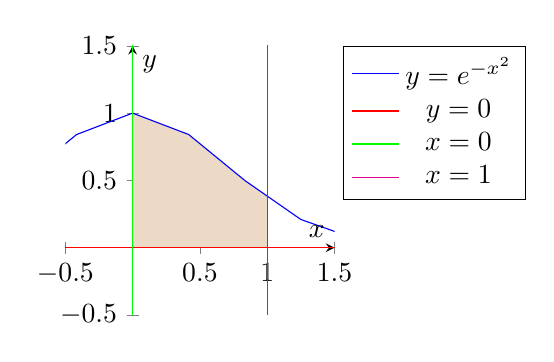
\begin{tikzpicture}
    \begin{axis}[xmin= -0.5, xmax= 1.5, ymin= -0.5, ymax= 1.5, width= 5cm, height= 5cm,
        xtick distance= 0.5, ytick distance = 0.5, xlabel=$x$, ylabel=$y$, axis lines=center,
        legend entries={$y=e^{-x^2}$, $y=0$, $x=0$, $x=1$},
        legend style={legend pos=outer north east} ]

        %\addplot[domain=x:x, mark]{};
        \addplot[name path=a, mark=none, blue]{ e^(-x^2) }; %y=e^{-x^2}
        \addplot[name path=b, mark=none, red](x,0); %y=0
        \addplot[mark=none, green](0,x); %x=0
        \addplot[mark=none, magenta](1,x); %x=1

        %Sombrear área
        \addplot fill between[ 
            of = a and b,
            soft clip = {domain = 0:1},
            %split, % calculate segments
            every even segment/.style = {brown!30},
            every odd segment/.style  = {brown!30}
        ];
    \end{axis}
\end{tikzpicture}

%Planteamiento (1)
%\textbf{Planteamiento:} \\
%\textit{Por discos...} \\
%$$\int_{a}^{b} x^2 dx$$ \\
%\textit{Por cilindros...} \\
%$$\int_{a}^{b} x^2 dx$$

\end{multicols}

%Solución (1)


% 2 ----------------------------------------------------------------------------------------------
\item Encuentra el volumen del sólido formado por la región encerrada por las curvas $y=x^2 +1$,
      $y=x+3$ al rotar alrededor del eje $y = -1$.

%Gráfica (2)
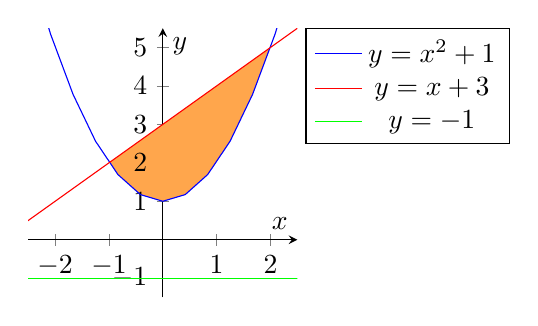
\begin{tikzpicture}
    \begin{axis}[xmin= -2.5, xmax= 2.5, ymin= -1.5, ymax= 5.5, width= 5cm, height= 5cm,
        xtick distance= 1, ytick distance = 1, xlabel=$x$, ylabel=$y$, axis lines=center,
        legend entries={$y=x^2 +1$, $y=x+3$, $y = -1$},
        legend style={legend pos=outer north east} ]

        %\addplot[domain=x:x, mark]{};
        \addplot[name path=a, mark=none, blue]{ x^(2) + 1 }; %y=x^2 +1
        \addplot[name path=b, mark=none, red]{ x+3 }; %y=x+3
        \addplot[mark=none, green](x,-1); %y = -1

        %Sombrear área
        \addplot fill between[ 
            of = a and b,
            soft clip = {domain = -1:2},
            split, % calculate segments
            every even segment/.style = {orange!70},
            every odd segment/.style  = {brown!30}
        ];
    \end{axis}
\end{tikzpicture}

%Solución (2)


% 3 ----------------------------------------------------------------------------------------------
\item Encuentra el volumen del sólido generado al hacer rotar alrededor de la recta $y=2$ la región
      acotada por las curvas $y = \sec x$, $y = 0$, $0 \leq x \leq \pi/3$.

%Gráfica (3)
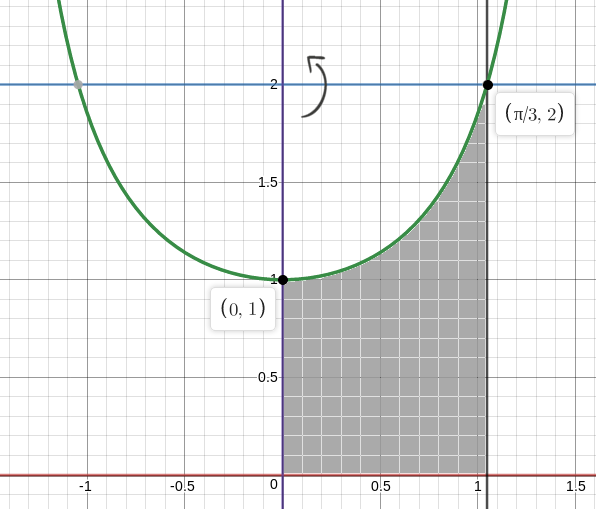
\includegraphics[width=5cm]{Images/grafica3.png}

%Solución (3)


% 4 ----------------------------------------------------------------------------------------------
\item Halla el volumen del sólido de revolución generado al hacer rotar la región acotada por las
      curvas $y = x^2$, $y = 4x - x^2$ , en torno a la recta $x = 2$.

%Gráfica (4)
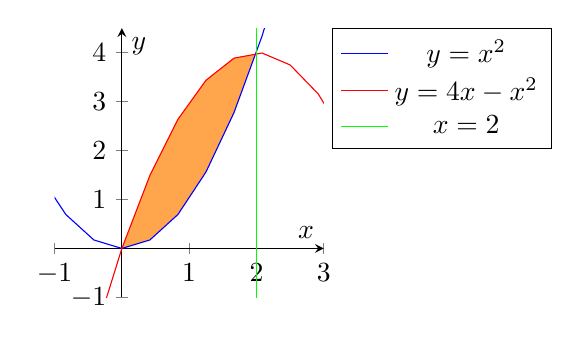
\begin{tikzpicture}
    \begin{axis}[xmin= -1, xmax= 3, ymin= -1, ymax= 4.5, width= 5cm, height= 5cm,
        xtick distance= 1, ytick distance = 1, xlabel=$x$, ylabel=$y$, axis lines=center,
        legend entries={$y=x^2$, $y=4x - x^2$, $x = 2$},
        legend style={legend pos=outer north east} ]

        %\addplot[domain=x:x, mark]{};
        \addplot[name path=a, mark=none, blue]{ x^2 }; %y=x^2
        \addplot[name path=b, mark=none, red]{ 4*x - x^2 }; %y=4x - x^2
        \addplot[mark=none, green](2,x); %x = 2

        %Sombrear área
        \addplot fill between[ 
            of = a and b,
            soft clip = {domain = 0:2},
            split, % calculate segments
            every even segment/.style = {orange!70},
            every odd segment/.style  = {brown!30}
        ];
    \end{axis}
\end{tikzpicture}

%Solución (4)


% 5 ----------------------------------------------------------------------------------------------
\item Determina el volumen de la región encerrada entre las curvas $y = 1 + x^2$ y $y = 0$ al rotar
      alrededor del eje $x$ cuando $0 \leq x \leq 2$.

%Gráfica (5)
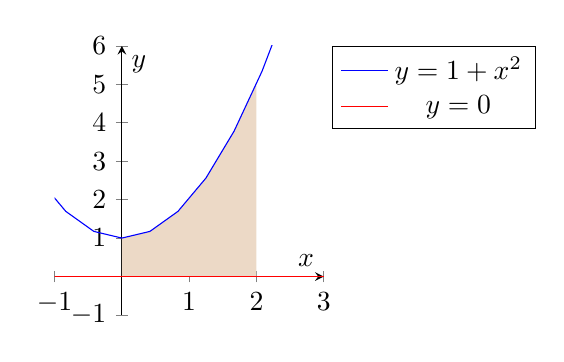
\begin{tikzpicture}
    \begin{axis}[xmin= -1, xmax= 3, ymin= -1, ymax= 6, width= 5cm, height= 5cm,
        xtick distance= 1, ytick distance = 1, xlabel=$x$, ylabel=$y$, axis lines=center,
        legend entries={$y=1+x^2$, $y=0$},
        legend style={legend pos=outer north east} ]

        %\addplot[domain=x:x, mark]{};
        \addplot[name path=a, mark=none, blue]{ 1 + x^2 }; %y=1+x^2
        \addplot[name path=b, mark=none, red](x,0); %y=0

        %Sombrear área
        \addplot fill between[ 
            of = a and b,
            soft clip = {domain = 0:2},
            %split, % calculate segments
            every even segment/.style = {brown!30},
            every odd segment/.style  = {brown!30}
        ];
    \end{axis}
\end{tikzpicture}

%Solución (5)


% 6 ----------------------------------------------------------------------------------------------
\item Determina el volumen de la región encerrada por la función $x = \sqrt{\sin y}$ con
      $0 \leq y \leq \pi$ y $x = 0$ si rota en $y = 4$.

%Gráfica (6)
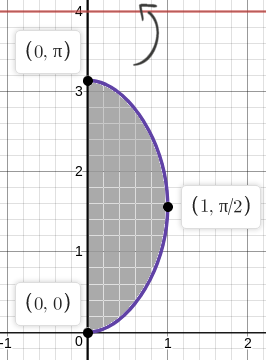
\includegraphics[height=5cm]{Images/grafica5.png}

%Solución (6)


% 7 ----------------------------------------------------------------------------------------------
\item Determinar la superficie del sólido de revolución generado al rotar en el eje $y$ la región
      definida por $y = x^3$ con $0 \leq x \leq 1$.

%Gráfica (7)
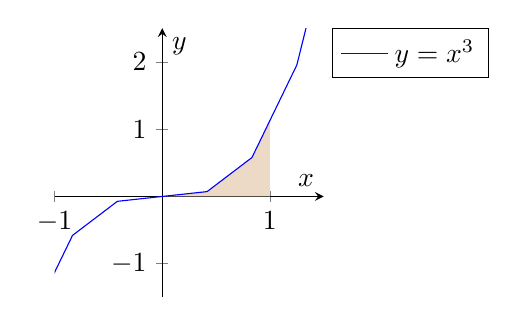
\begin{tikzpicture}
    \begin{axis}[xmin= -1, xmax= 1.5, ymin= -1.5, ymax= 2.5, width= 5cm, height= 5cm,
        xtick distance= 1, ytick distance = 1, xlabel=$x$, ylabel=$y$, axis lines=center,
        legend entries={$y=x^3$},
        legend style={legend pos=outer north east} ]

        %\addplot[domain=x:x, mark]{};
        \addplot[name path=a, mark=none, blue]{ x^3 }; % y=x^3
        \addplot[name path=b, draw=none](x,0);

        Sombrear área
        \addplot fill between[ 
            of = a and b,
            soft clip = {domain = 0:1},
        %    %split, % calculate segments
            every even segment/.style = {brown!30},
            every odd segment/.style  = {brown!30}
        ];
    \end{axis}
\end{tikzpicture}

%Solución (7)


\end{enumerate}

\end{document}